La figura de este ejercicio representa dos bolas de billar, $A$ y $B$, que inicialmente se mueven con cantidades de movimiento $q_A$ = 2.5 kg$\cdot$m/s y $q_B$ = 1.5 kg$\cdot$m/s. La bola $A$ alcanza a la bola $B$ y después del choque, pasan a moverse con cantidades de movimiento $\Vec{q\small'}_{\!\!A}$ y $\Vec{q'}_{\!\!B}$, como muestra la figura. Considerando el sistema constituido por las dos bolas, responda:
\begin{enumerate}
    \item ¿Cuál es la cantidad de movimiento inicial del sistema?
    \item Las fuerzas que las bolas ejercen una sobre la otra durante el choque, ¿son internas o externas?
    \item Suponiendo que la resultante de las fuerzas externas es nula, ¿cuál es el valor de la cantidad de movimiento final del sistema?
    \item Sabiendo que $q'_A$ = 1.0 kg$\cdot$m/s, ¿cuál es el valor de $q'_B$?
    \item Suponiendo que la masa de $B$ es de 0.50 kg, ¿cuál es el valor de la velocidad final de esta bola?
\end{enumerate}
\begin{figure}[htb]
  \centering
  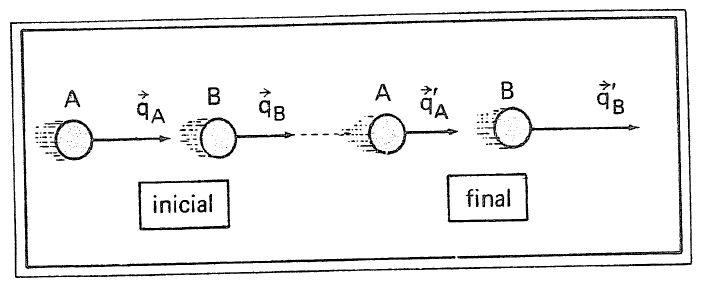
\includegraphics[scale=0.4]{figuras/fig_alvarenga_p414_15.png}
  \caption{Problema 8}
\end{figure}
